\definecolor{LightCyan}{rgb}{0.88,1,1}
\definecolor{LightYellow}{rgb}{255,255,0}
\tikzstyle{vecArrow} = [thick, decoration={markings,mark=at position
	1 with {\arrow[semithick]{open triangle 60}}},
double distance=2pt, shorten >= 5.5pt,
preaction = {decorate},
postaction = {draw,line width=1.4pt, white,shorten >= 4.5pt}]
\tikzstyle{innerWhite} = [semithick, white,line width=1.4pt, shorten >= 4.5pt]


\newcommand*{\sdd}{\tikz \draw [baseline, fill=red,draw=red,circular drop shadow] circle (2pt);}
\newcommand*{\sdv}{\tikz \draw [baseline, fill=green,draw=green,circular drop shadow] circle (2pt);}

\section{Resumen }
\subsection{Estructuras y c\'alculos n\'umericos}
\begin{frame}[t]
\frametitle{Estructuras y c\'alculos n\'umericos }
\framesubtitle{}
\vspace{-0.5cm}




\begin{tikzpicture}[remember picture, overlay]
\node<1->[anchor = north west, text width = 5cm, yshift = -0.7cm](txt) at (current page.north west) {
	\begin{tcolorbox}[enhanced,title = Trabajo Realizado,
	fonttitle=\bfseries,
	left=1mm,
	top=1mm,
	bottom=1mm,
	right=1mm,
	width = 5cm,
	height=2.25cm,
	boxsep = 0cm,
	coltitle=green!25!black,
	attach boxed title to top center={yshift=-2mm,yshifttext=-1mm},
	boxed title style={colframe=green!75!black,
		colback=yellow!50!green}]
	\begin{itemize}
	\fontsize{8}{1}\selectfont
	\item<1-> Estudio de estructuras de Pozos cu\'anticos acoplados
	\item<3-> C\'alculos n\'umericos
	\end{itemize}
	\end{tcolorbox}	
};


\node<1->[anchor= north east,xshift=-2cm,yshift=-0.2cm](st) at (current page.north east){\includegraphics[scale=0.25]{Figures/STRUCTURES/FIG1}};

\node<2>[xshift = -1cm,yshift=-2.5cm,scale=0.97](sq) at (current page.center){
	\begin{tabular}{cccc} \toprule
	Sample number                     & Well width $d_{1} (nm)$ &Well width $d_{2} (nm)$ & Tipo de Dopaje  \\ \midrule
	\rowcolor{LightCyan}
	S1    & 11.87        & 11.87     & n  \\ 	
    A1    & 13.85        & 11.87     & n\\ 	
    A2    & 23.74        & 11.87     & n \\
   \rowcolor{LightYellow}
	A3	  & 23.74        & 11.87     & p \\
     \bottomrule
	\end{tabular}
};


\node<4-8>[anchor= north,yshift=0mm,blue](ef) at (txt.south){$\mathbf{k\cdot p}$ Luttinger-Kohn's model };





\node<4-8>[anchor= north,xshift=0.8cm,yshift=3mm] at (st.south){\includegraphics[scale=0.25]{Figures/SYMMETRY/BBULK}};

\node<5-8>[xshift=1cm,yshift=-1cm,scale=0.825](e1) at (ef.south) {
	$\begin{aligned}
	%H^{e,h}\psi(x) = E^{e,h}\psi(x).
\onslide<5-8>{&\left\lbrace \dfrac{p^2}{2m_{0}}+V\mathbf{(r)}+\dfrac{\hbar}{m_0}\mathbf{k\cdot p}+\dfrac{\hbar}{4m_{0}^{2}c^2}\left[\nabla V\times\mathbf{p}\right]\cdot\mathbf{\sigma} +\dfrac{\hbar}{4m_{0}^{2}c^2}\nabla V\times \mathbf{k\cdot\sigma}\right\rbrace}\\
&\times u_{nk}\mathbf{(r)}=E'u_{nk}\mathbf{(r)}
%\onslide<5->{Hu_{k}\mathbf{(r)}&=E\mathbf{(k)}u_{k}\mathbf{(r)}\\
%\onslide<6->{H=\left[\dfrac{p^2}{m_{0}}+\dfrac{\hbar}{m_{0}}\mathbf{k\cdot p}\right] u_{nk}\mathbf{(r)}&=\left[E_{n}\mathbf{(k)}-\dfrac{\hbar^2 k^2}{2m_{0}}\right]u_{nk}\mathbf{(r)}}
	\end{aligned}$
	    };
	    
\node<6->[xshift=1cm,yshift=-1.7cm,scale=0.825,anchor=north](e2) at (ef.south) {
	$\begin{aligned}
\onslide<6-8>{Hu_{nk}\mathbf{(r)}&=E\mathbf{(k)}u_{nk}\mathbf{(r)}}\\
\onslide<7-8>{H&= H_{0} +\dfrac{\hbar^2k^2}{2m_{0}} + \dfrac{\hbar}{4m_{0}^{2}c^2} \nabla V\times \mathbf{p\cdot \sigma} + H' }
	\end{aligned}$
	    };
    
\node<8>[xshift=-1.1cm,yshift=-0.1cm,scale=0.825,anchor=north west](e3) at (e2.south west) {
	$
    H = - \begin{pmatrix}
    P+Q      & -S   		 &  R    	     & 0          &  -S/\sqrt{2}    &  \sqrt{2}R\\
    -S^{+}   &  P-Q 		 &  0  		     & R          & -\sqrt{2}Q      & \sqrt{3/2} S\\
    R^{+}    &   0  		 & P-Q 		     & S          & \sqrt{3/2}S^{+} & \sqrt{2}Q  \\
    0        &  R^+ 		 & S^+           & P+Q        & -\sqrt{2}R^+    &-S^+ /\sqrt{2}\\
-S^+/\sqrt{2}& -\sqrt{2}Q^{+}&  \sqrt{3/2}S  & -\sqrt{2}R & P+\Delta        & 0\\
\sqrt{2}R    & \sqrt{3/2}S^+ &\sqrt{2}Q^+    & -S/\sqrt{2}& 0				& P+\Delta \\   
\end{pmatrix}
$
	    };


%
\node<9->[anchor= north,yshift=0mm,blue](ef) at (txt.south){Effective Mass Approach};
\node<9->[anchor= north,xshift=0.8cm,yshift=3mm] at (st.south){\includegraphics[scale=0.25]{Figures/SYMMETRY/BQWS}};
\node<10->[xshift=0.5cm,yshift=-1cm] at (ef.south) {
	$\begin{aligned}
	%H^{e,h}\psi(x) = E^{e,h}\psi(x).
	\displaystyle\left[- \dfrac{\hbar^{2}}{2m_{jz}}\dfrac{d^{2}}{dz^{2}}+V(z)\displaystyle\right]\psi_{nj}(z) &= E_{nj}\psi_{nj}(z),\\
	j&=e,H,L.
	\end{aligned}$
	    };
    
\node<10->[yshift=-3.8cm] at (txt.south){
\animategraphics[autoplay,loop,width=4cm]{1}{FIGURES/MESH/MESH}{0}{5}};

\end{tikzpicture}





\end{frame}

\subsection{Reducción de simetría y\\ Modelo Perturbativo}
\begin{frame}{Modelo de anisotropía}{
\only<1-4>{Reducción de simetría $D_{2d} \rightarrow C_{2v}$}
\only<5->{Modelo Perturbativo }}
\begin{tikzpicture}[remember picture, overlay]
\node<1-4>[anchor=north west,yshift=-10mm,xshift=2mm,text width=8cm, scale=0.9, align=justify,inner sep=0mm](p) at (current page.north west) {
	\begin{tcolorbox}[
	colback=green!5!white,
	colframe=blue!75!black,sharp corners,
	rounded corners=northwest ]
	Pierre Curie:
la ruptura de la simetría tiene la siguiente función: para que se produzca un fenómeno en un medio, el grupo de simetría original del medio debe ser reducido (roto, en la terminología actual) al grupo de simetría del fenómeno (o a un subgrupo del grupo de simetría del fenómeno) por la acción de alguna causa. 
	\end{tcolorbox}
	};

\node<2->[anchor=north,
draw,
fill=green!70!white,
scale=1.5,
xshift=18mm,
yshift=-8mm](s1) at (current page.north) {$T_{d}$};

\node<2->[anchor= north](b) at(s1.south){GaAs(001) Bulto };

\node<3->[anchor=north,
draw,
fill=green!70!white,
xshift=0cm,
yshift=-1cm,
scale=1.5](s2) at (s1.south) {$D_{2d}$};
\node<3->[anchor= north](sqws) at(s2.south){GaAs QWs sim\'etricos };


\node<4->[anchor=north,
draw,
fill=green!70!white,
yshift=-1cm,
scale=1.5](s3) at (s2.south) {$C_{2v}$};
\node<4->[anchor= north] at(s3.south){Pozos GaAs asimetricos  };



\draw<3->[vecArrow] (b) to (s2);
\draw<4->[vecArrow] (sqws) to (s3);

\node<3>[anchor=south west,yshift=0mm] (f1) at (current page.west) {PCA simetricos $d_{1} = d_{2}$};
\node<3>[anchor=north west](i1) at (f1.south west) {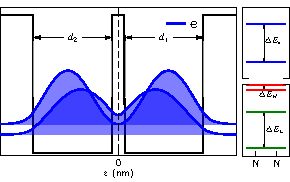
\includegraphics[width=0.7\linewidth]{Figures/WELLS-PLOTS/M4_3523/M4_3523-IOA}};
%
\node<4>[anchor=south west, yshift=0mm] (f2) at (current page.west) {PCA asimetricos $d_{1} > d_{2}$};
\node<4->[anchor=south west](i2) at (current page.south west) {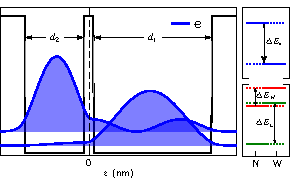
\includegraphics[width=0.7\linewidth]{Figures/WELLS-PLOTS/M4_3521/M4_3521-IOA}};


\node<5->[text width=\textwidth,anchor=north west,align=justify, blue,yshift=-0.8cm](tt1) at (current page.north west){``La reduccion de sim\'etria (ruptura) tiene como consecuencia  la mezcla  los huecos-  pesados y ligeros''};


\node<6->[anchor=north, yshift=-1mm,xshift=-5mm, text width=22mm,scale=1.5,align=center,blue,draw](e1) at (tt1.south){
	$\begin{aligned}
	\langle \psi_{\rm{hhn}}| \mathcal{H} | \psi_{\rm{lhn}} \rangle
	\end{aligned}$
};

\node<7->[anchor=north, scale=1.2,yshift=-3mm, blue](e2) at (e1.south) {
	$\begin{aligned}
	\dfrac{
	       \langle \psi_{\rm{en}} | \psi_{\rm{hhn}} \rangle
	       \langle \psi_{\rm{hhn}}| \mathcal{H} | \psi_{\rm{lhn}} \rangle
	       \langle\psi_{\rm{lhn}} | \psi_{\rm{en}} \rangle
	      }
	      {\rm{\Delta E_{n}}
	      }
	\end{aligned}$};
	
\node<8->[anchor=north,yshift=-1mm,scale=1.25,blue](e3) at (e2.south) {
	$\begin{aligned}
	\mathbf{\mathrm{\Delta E = E_{_{hhn}}-E_{_{lhn}}}}
	\end{aligned}$};
\end{tikzpicture}

\end{frame}


\subsection{Resultados num\'ericos}
\begin{frame}[t]{Resultados num\'ericos}
\framesubtitle{Muestra \only<1>{S1} \only<2>{A2}  }
\begin{tikzpicture}[remember picture, overlay]
\node<1>[anchor=north,yshift=-7mm,xshift=-10mm] at (current page.north){\includegraphics[width=0.9\textwidth]{/mnt/d/OneDrive - Universidad Autonoma de San Luis Potosi - UASLP/Documentos/RUCO/ANALISIS/M4_3523/PLOTS/PLOT-M4_3523-PAPER/Fig_2a}};
\node<2->[anchor=north,yshift=-7mm,xshift=-10mm] at (current page.north){\includegraphics[width=0.9\textwidth]{/mnt/d/OneDrive - Universidad Autonoma de San Luis Potosi - UASLP/Documentos/RUCO/ANALISIS/M4_3521/PLOTS/PLOT-M4_3521-PAPER/Fig_2b}};


\node[anchor=south,scale=1,xshift=-10mm,yshift=2mm] at (current page.south){\includegraphics[width=\textwidth]{./Figures/TABLE/TABLE.pdf}};
\end{tikzpicture}
\end{frame}


\subsection{Resultados experimentales RAS}

\begin{frame}[t]{Resultados experimentales}



\begin{tikzpicture}[remember picture, overlay]
\foreach [count=\xi from 1]\x in {1,...,3}{
\node<\xi->[anchor=south west,yshift=-2mm,xshift=-1.5mm](p1) at (current page.south west) {\includegraphics[page={\x},width=0.495\linewidth]{Figures/RAS/Fig_3}};
}

%\node<4->[anchor=north west,text width=3.5cm,xshift=-3.5mm,draw=blue,color=red](tiao) at (p1.north east){IOA  inducida por campo\\ instrinseco?};


\foreach [count=\xi from 5]\x in {1,...,3}{
	\node<\xi>[anchor=north west,xshift=-2mm](p2) at (p1.north east) {\includegraphics[page={\x},width=0.53\linewidth]{Figures/RAS/Fig_5-A}};
}

\node<7->[anchor=north,yshift=2mm] at (p2.south) {\includegraphics[width=0.53\linewidth]{Figures/RAS/Fig_4}};
\end{tikzpicture}
\end{frame}



\begin{frame}[t]{Resultados experimentales}

\begin{tikzpicture}[remember picture, overlay]
\node[anchor=center,xshift=-10mm] at (current page.center) {\includegraphics[width=\textwidth]{Figures/PAPER/AC}};
\end{tikzpicture}
\end{frame}
